\graphicspath{ {images/} }

\titledquestion{Attention Exploration}[14]
\label{sec:analysis}

Multi-head self-attention is the core modeling component of Transformers.
In this question, we'll get some practice working with the self-attention equations, and motivate why multi-headed self-attention can be preferable to single-headed self-attention.

Recall that attention can be viewed as an operation on a \textit{query} vector $q\in\mathbb{R}^d$, a set of \textit{value} vectors $\{v_1,\dots,v_n\}, v_i\in\mathbb{R}^d$, and a set of \textit{key} vectors $\{k_1,\dots,k_n\}, k_i \in \mathbb{R}^d$, specified as follows:
\begin{align}
&c = \sum_{i=1}^{n} v_i \alpha_i \\
&\alpha_i = \frac{\exp(k_i^\top q)}{\sum_{j=1}^{n} \exp(k_j^\top q)}
\end{align} 
with $alpha = \{\alpha_1, \ldots, \alpha_n\}$ termed the ``attention weights''. 
Observe that the output $c\in\mathbb{R}^d$ is an average over the value vectors weighted with respect to $\alpha$.

\begin{parts}

\part[3] \label{copying} \textbf{Copying in attention.} One advantage of attention is that it's particularly easy to ``copy'' a value vector to the output $c$. In this problem, we'll motivate why this is the case.

\begin{subparts}
    \subpart[2] The distribution $\alpha$ is typically relatively ``diffuse''; the probability mass is spread out between many different $\alpha_i$. However, this is not always the case. \textbf{Describe} (in one sentence) under what conditions the categorical distribution $\alpha$ puts almost all of its weight on some $\alpha_j$, where $j \in \{1, \ldots, n\}$ (i.e. $\alpha_j \gg \sum_{i \neq j} \alpha_i$). What must be true about the query $q$ and/or the keys $\{k_1,\dots,k_n\}$?

    \ifans{When the score $k_j^\top q$ is much larger than every other score $k_i^\top q$ for $i \neq j$ --- i.e.~when the query $q$ is strongly aligned with the key $k_j$ and (nearly) orthogonal to or negatively aligned with all the other keys --- the gap $k_j^\top q - \max_{i\neq j} k_i^\top q$ is large, and the exponentials inside the softmax make $\alpha_j$ dominate all the other weights, so $\alpha_j \to 1$.}

    \subpart[1] Under the conditions you gave in (i), \textbf{describe} the output $c$. 

    \ifans{Then $c \approx v_j$: since $\alpha_j \approx 1$ and $\alpha_i \approx 0$ for $i \neq j$, the output of attention is essentially the value vector $v_j$ itself --- attention ``copies'' $v_j$ to the output.}

\end{subparts}


\part[2]\textbf{An average of two.} 
\label{q_avg_of_two}
Instead of focusing on just one vector $v_j$, a Transformer model might want to incorporate information from \textit{multiple} source vectors.

Consider the case where we instead want to incorporate information from \textbf{two} vectors $v_a$ and $v_b$, with corresponding key vectors $k_a$ and $k_b$.
Assume that (1) all key vectors are orthogonal, so $k_i^\top k_j = 0$ for all $i \neq j$; and (2) all key vectors have norm $1$.
\textbf{Find an expression} for a query vector $q$ such that $c \approx \frac{1}{2}(v_a + v_b)$, and \textbf{justify your answer}.\footnote{Hint: while the softmax function will never \textit{exactly} average the two vectors, you can get close by using a large scalar multiple in the expression.} (Recall what you learned in part~(\ref{copying}).)

\ifans{
Choose $q = \lambda(k_a + k_b)$ for a large scalar $\lambda > 0$. Because the keys are orthonormal, $k_i^\top q = \lambda\left(k_i^\top k_a + k_i^\top k_b\right)$ equals $\lambda$ for $i \in \{a, b\}$ and $0$ for all other $i$. The attention weights are therefore
\[
\alpha_a = \alpha_b = \frac{e^{\lambda}}{2e^{\lambda} + (n-2)} \ \xrightarrow{\ \lambda \to \infty\ } \ \frac{1}{2}, \qquad \alpha_i \xrightarrow{\ \lambda \to \infty\ } 0 \quad (i \notin \{a,b\}),
\]
so $c = \sum_{i=1}^{n} \alpha_i v_i \approx \frac{1}{2}(v_a + v_b)$, and the approximation becomes exact as $\lambda \to \infty$.
}

\part[5]\textbf{Drawbacks of single-headed attention:} \label{q_problem_with_single_head}
In the previous part, we saw how it was \textit{possible} for a single-headed attention to focus equally on two values.
The same concept could easily be extended to any subset of values.
In this question we'll see why it's not a \textit{practical} solution.

Consider a set of key vectors $\{k_1,\dots,k_n\}$ that are now randomly sampled, $k_i\sim \mathcal{N}(\mu_i, \Sigma_i)$, where the means $\mu_i \in \mathbb{R}^d$ are known to you, but the covariances $\Sigma_i$ are unknown (unless specified otherwise in the question).
Further, assume that the means $\mu_i$ are all perpendicular; $\mu_i^\top \mu_j = 0$ if $i\not=j$, and unit norm, $\|\mu_i\|=1$.

\begin{subparts}
\subpart[2] Assume that the covariance matrices are $\Sigma_i = \alpha I, \forall i \in \{1, 2, \ldots, n\}$, for vanishingly small $\alpha$.
Design a query $q$ in terms of the $\mu_i$ such that as before, $c\approx \frac{1}{2}(v_a + v_b)$, and provide a brief argument as to why it works.

\ifans{
Take $q = \lambda(\mu_a + \mu_b)$ for a large $\lambda > 0$. With $\Sigma_i = \alpha I$ for vanishingly small $\alpha$, every sampled key is a tiny perturbation of its mean, $k_i \approx \mu_i$. Hence, by the orthogonality and unit norm of the $\mu_i$, we get $k_a^\top q \approx \lambda$ and $k_b^\top q \approx \lambda$ while $k_i^\top q \approx 0$ for $i \notin \{a, b\}$, with errors of size $O(\sqrt{\alpha})$. Exactly as in part~(\ref{q_avg_of_two}), the softmax then concentrates almost all of its mass, equally, on $a$ and $b$, giving $c \approx \frac{1}{2}(v_a + v_b)$.
}

\subpart[3] Though single-headed attention is resistant to small perturbations in the keys, some types of larger perturbations may pose a bigger issue. In some cases, one key vector $k_a$ may be larger or smaller in norm than the others, while still pointing in the same direction as $\mu_a$.\footnote{Unlike the original Transformer, newer Transformer models apply layer normalization before attention. In these pre-layernorm models, norms of keys cannot be too different which makes the situation in this question less likely to occur.}

As an example, let us consider a covariance for item $a$ as $\Sigma_a = \alpha I + \frac{1}{2}(\mu_a\mu_a^\top)$ for vanishingly small $\alpha$ (as shown in figure \ref{ka_plausible}). This causes $k_a$ to point in roughly the same direction as $\mu_a$, but with large variances in magnitude. Further, let $\Sigma_i = \alpha I$ for all $i \neq a$.
\begin{figure}[h]
\centering
\captionsetup{justification=centering,margin=2cm}
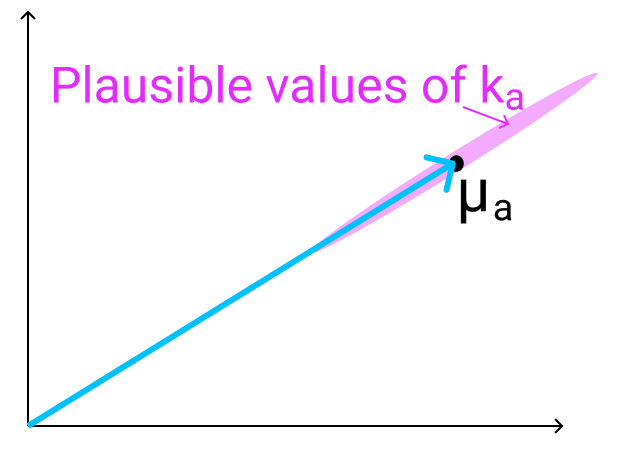
\includegraphics[width=0.35\linewidth]{images/ka_plausible.png}
\caption{The vector $\mu_a$ (shown here in 2D as an example), with the range of possible values of $k_a$ shown in red. As mentioned previously, $k_a$ points in roughly the same direction as $\mu_a$, but may have larger or smaller magnitude.}
\label{ka_plausible}
\end{figure}

When you sample $\{k_1,\dots,k_n\}$ multiple times, and use the $q$ vector that you defined in part i., what do you expect the vector $c$ will look like qualitatively for different samples? Think about how it differs from part (i) and how $c$'s variance would be affected.

\ifans{
Now $k_a$ has a large variance along its own mean direction: $\mathrm{Var}\left(k_a^\top \mu_a\right) = \mu_a^\top \Sigma_a \mu_a = \alpha + \tfrac{1}{2} \approx \tfrac{1}{2}$, so $k_a^\top \mu_a$ fluctuates around $1$ with standard deviation $\approx 1/\sqrt{2}$, whereas $k_b^\top \mu_b \approx 1$ is stable. The two scores that compete in the softmax are $k_a^\top q = \lambda\,(k_a^\top \mu_a)$ and $k_b^\top q \approx \lambda$, so their difference $\lambda\left(k_a^\top \mu_a - 1\right)$ is random with standard deviation $\approx \lambda/\sqrt{2}$, which is huge because $\lambda$ is large. Since softmax amplifies score differences exponentially, whenever $k_a^\top \mu_a > 1$ we get $c \approx v_a$, whenever $k_a^\top \mu_a < 1$ we get $c \approx v_b$, and near-equal scores (which would give $\approx \frac{1}{2}(v_a + v_b)$) are rare. So, across samples, $c$ no longer stably equals $\frac{1}{2}(v_a + v_b)$ as in part~(i); instead it has very large variance, flipping between $\approx v_a$ and $\approx v_b$.
}
\end{subparts}

\part[3]\textbf{Benefits of multi-headed attention:} \label{q_multi_head}
Now we'll see some of the power of multi-headed attention.
We'll consider a simple version of multi-headed attention which is identical to single-headed self-attention as we've presented it, except two query vectors ($q_1$ and $q_2$) are defined, which leads to a pair of vectors ($c_1$ and $c_2$), each the output of single-headed attention given its respective query vector.
The final output of the multi-headed attention is their average, $\frac{1}{2}(c_1+c_2)$.

As in question 1(\ref{q_problem_with_single_head}), consider a set of key vectors $\{k_1,\dots,k_n\}$ that are randomly sampled, $k_i\sim \mathcal{N}(\mu_i, \Sigma_i)$, where the means $\mu_i$ are known to you, but the covariances $\Sigma_i$ are unknown.
Also as before, assume that the means $\mu_i$ are mutually orthogonal; $\mu_i^\top \mu_j = 0$ if $i\not=j$, and unit norm, $\|\mu_i\|=1$.

\begin{subparts}
\subpart[1]
Assume that the covariance matrices are $\Sigma_i=\alpha I$, for vanishingly small $\alpha$.
Design $q_1$ and $q_2$ in terms of $\mu_i$ such that $c$ is approximately equal to $\frac{1}{2}(v_a+v_b)$. 
Note that $q_1$ and $q_2$ should have different expressions.

\ifans{
Choose $q_1 = \lambda \mu_a$ and $q_2 = \lambda \mu_b$ with large $\lambda > 0$ (so $q_1 \neq q_2$). For head 1, only key $a$ has a large score ($k_a^\top q_1 \approx \lambda$; all others $\approx 0$), so $c_1 \approx v_a$. For head 2, only key $b$ has a large score ($k_b^\top q_2 \approx \lambda$), so $c_2 \approx v_b$. Their average is therefore $c = \tfrac{1}{2}(c_1 + c_2) \approx \tfrac{1}{2}(v_a + v_b)$.
}

\subpart[2]
Assume that the covariance matrices are $\Sigma_a=\alpha I + \frac{1}{2}(\mu_a\mu_a^\top)$ for vanishingly small $\alpha$, and $\Sigma_i=\alpha I$  for all $i \neq a$.
Take the query vectors $q_1$ and $q_2$ that you designed in part i.
What, qualitatively, do you expect the output $c$ to look like across different samples of the key vectors? Explain briefly in terms of variance in $c_1$ and $c_2$. You can ignore cases in which $k_a^\top q_i < 0$.

\ifans{
Head 1 uses $q_1 = \lambda \mu_a$, so its only nonzero score is $k_a^\top q_1 = \lambda\,(k_a^\top \mu_a)$, which remains positive (we ignore the negative cases). No matter how the magnitude of $k_a$ fluctuates, all other scores are $\approx 0$, so the softmax still concentrates on $a$: $c_1 \approx v_a$ for every sample, with small variance --- the fluctuation only changes how sharply peaked $\alpha_1$ is, not \emph{which} value is copied. Head 2 uses $q_2 = \lambda \mu_b$; key $b$ is unperturbed ($\Sigma_b = \alpha I$), so $c_2 \approx v_b$ with small variance as well. Since the two heads produce independent, stable outputs, the average $c = \tfrac{1}{2}(c_1 + c_2) \approx \tfrac{1}{2}(v_a + v_b)$ is stable across samples: the variance of $c$ is small (it is $\tfrac{1}{4}\left(\mathrm{Var}(c_1) + \mathrm{Var}(c_2)\right)$), unlike the single-head case in part~(\ref{q_problem_with_single_head})(ii).
}
\end{subparts}

\part[1] Based on part~(\ref{q_multi_head}), briefly summarize how multi-headed attention overcomes the drawbacks of single-headed attention that you identified in part~(\ref{q_problem_with_single_head}).

\ifans{
The drawback of single-headed attention is that one query must be aligned with \emph{several} keys at once, so a perturbation of any attended key's norm is exponentially amplified by the softmax and the output becomes unstable (part~(c)(ii)). Multi-headed attention decomposes the desired combination into separate heads, each with its own query aligned to a \emph{single} key direction: each head's attention then concentrates on one value regardless of how that key's norm fluctuates (low variance per head), and averaging the stable heads produces the desired mixture $\frac{1}{2}(v_a + v_b)$ with greatly reduced variance.
}

\end{parts}
